\documentclass[11pt]{article}
\usepackage{graphicx}
\usepackage{fullpage}
\usepackage{amsfonts}
\usepackage{amssymb}
\usepackage{amsmath}
\usepackage{xcolor}
\usepackage{algorithm}
\usepackage{algorithmic}
\usepackage{enumitem}
\usepackage{fourier}
\usepackage[normalem]{ulem}


\newcommand{\F}{\mathbb{F}}
\newcommand{\np}{\mathop{\rm NP}}
%\newcommand{\binom}[2]{{#1 \choose #2}}

\newcommand{\mnote}[1]{{\color{red} [Madhu: #1]}}
\newcommand{\achnote}[1]{{\color{orange} [Sitan: #1]}}

\newcommand{\Z}{{\mathbb Z}}
\newcommand{\vol}{\mathop{\rm Vol}}
\newcommand{\conp}{\mathop{\rm co-NP}}
\newcommand{\atisp}{\mathop{\rm ATISP}}
\renewcommand{\vec}[1]{{\mathbf #1}}
\newcommand{\cupdot}{\mathbin{\mathaccent\cdot\cup}}
\newcommand{\mmod}[1]{\ (\mathrm{mod}\ #1)}

\setlength{\parskip}{\medskipamount}
\setlength{\parindent}{0in}

\begin{document}

%{\color{brown} Changes after test solvers started looking indicated in brown.}

%{\color{red} Changes after release indicated in red.}

        \section*{CS 124 Homework 2: Spring 2024}

%{\color{brown}        \sout{\textbf{Your name:}}}

        \textbf{Collaborators: }

        \textbf{No. of late days used on previous psets:} 0\\
        \textbf{No. of late days used after including this pset:} 0

Homework is due {\color{blue} Wednesday Feb 14 at 11:59pm ET}. {\color{brown} Note that although this is \emph{two} weeks from the date on which this is assigned, your first programming assignment will also be released on Feb 7, so you should budget your time appropriately.} You are allowed up to {\bf twelve} late days, but the number of late days you take on each assignment must be a nonnegative integer at most {\bf two}. 

Try to make your answers as clear and concise as possible;
style may count in your grades. Assignments must be submitted in pdf format on Gradescope. If you do assignments by hand, you will need to scan your papers to turn them in.


{\bf Collaboration Policy:} You may collaborate on this (and all problem sets) only with other students currently enrolled in the class, and of course you may talk to the Teaching Staff or use Ed. You may also consult the recommended books for the course and course notes linked from the timetable. You may not use Generative AI or large language models, or search the web for solutions, or post the questions on chat forums. Furthermore, you must follow the "one-hour rule" on collaboration.  You may not write anything that you will submit within one hour of collaborating with other students or using notes from such sources. That is, whatever you submit must first have been in your head alone, or notes produced by you alone, for an hour. Subject to that, you can collaborate with other students, e.g. in brainstorming and thinking through approaches to problem-solving.


For all homework problems where you are asked to give an algorithm, you must prove the correctness
of your algorithm and establish the best upper bound that you can give for the running time. Generally
better running times will get better credit; generally exponential-time algorithms (unless specifically asked
for) will receive no or little credit. You should always write a clear informal description of your algorithm
in English. You may also write pseudocode if you feel your informal explanation requires more precision
and detail, but keep in mind pseudocode does NOT substitute for an explanation. Answers that consist
solely of pseudocode will receive little or no credit. Again, try to make your answers clear and concise.

%There is a (short) programming problem on this assignment; you {\bf should \textit{NOT} code} with others on this problem like you will for the ``major'' programming assignments later in the course. (You may talk about the problem, as you can for other problems.)

\section*{Problems}

\begin{enumerate}
\item 
\begin{enumerate}
\item 
{\bf (7 points)}
We saw in lecture that we can find a topological sort of a directed acyclic graph by running DFS
and ordering according to the postorder time
(that is, we add a vertex to the sorted list \emph{after} we visit its out-neighbors).
Suppose we try to build a topological sort by ordering in increasing order according to the preorder, and 
not the postorder, time.  Give a counterexample to show this doesn't work, and explain why it's a counterexample.  

\begin{quote}
  \color{purple}
  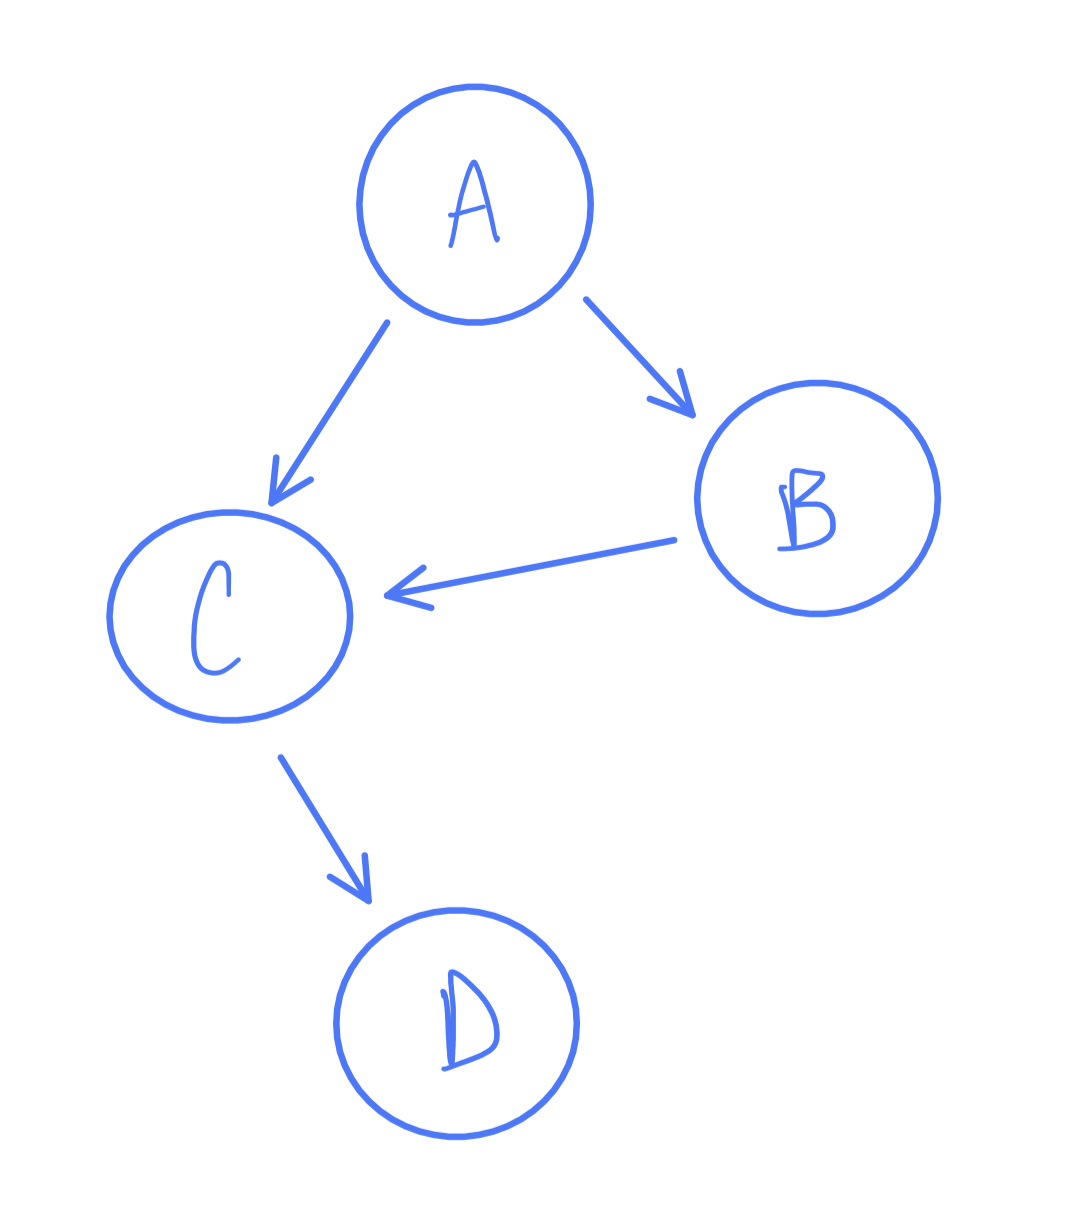
\includegraphics[width=0.6\linewidth]{"./pics/q1_graph.png"}

  \medskip
  Let the graph above represent precedence relations where $A$ has no restrictions, $B$ must come after $A$, $C$ must come after $A$ and $B$, and $D$ must come after $C$. 

  \medskip
  Consider a possible depth-first traversal of this graph starting at $A$. In the preorder list, $(X, X)$ indicates a vertex and the time it is visited beginning at zero: $(A, 0), (C, 1), (D, 2), (B, 3)$. 

  \medskip
  Sorting this by increasing preorder time yields an invalid topological sort of $A \rightarrow C \rightarrow D \rightarrow B$. This is not a valid topological sorting because $B$ must come before $C$ and here it is not.
  
\end{quote}

\item 
{\bf (7 points)}
Same as above, but we try to sort by decreasing preorder time.
\begin{quote}
  \color{purple}
  Consider the same graph as above and the same search path as above: $(A, 0), (C, 1), (D, 2), (B, 3)$.

  \medskip
  Sorting this by decreasing preorder time yields an invalid topological sort of $B \rightarrow D \rightarrow C \rightarrow A$. This is not a valid  topological sorting because $A$ must come before $B$ and $C$ but here it does not.
\end{quote}

\end{enumerate}


\item
{\bf (15 points)}
The {\em risk-free currency exchange problem} offers a risk-free way
to make money.  Suppose we have currencies $c_1,\ldots,c_n$.  (For
example, $c_1$ might be dollars, $c_2$ rubles, $c_3$ yen, etc.)  For
various pairs of distinct currencies $c_i$ and $c_j$ (but not
necessarily every pair!) there is an exchange rate $r_{i,j}$ such that
you can exchange one unit of $c_i$ for $r_{i,j}$ units of $c_j$.
(Note that even if there is an exchange rate $r_{i,j}$, so it is possible to
turn currency $i$ into currency $j$ by an exchange, the reverse might not
be true--- that is, there might
not be an exchange rate $r_{j,i}$.)  Now if, because of exchange rate
strangeness, $r_{i,j} \cdot r_{j,i} > 1$, then you can make money
simply by trading units of currency $i$ into units of currency $j$ and
back again.  (At least, if there are no exchange costs.)  This almost
never happens, but occasionally (because the updates for exchange
rates do not happen quickly enough) for very short periods of time
exchange traders can find a sequence of trades that can make risk-free
money.  That is, if there is a sequence of currencies
$c_{i_1},c_{i_2},\ldots,c_{i_k}$ such that $r_{{i_1},{i_2}} \cdot
r_{{i_2},{i_3}} \ldots \cdot r_{{i_{k-1}},{i_k}} \cdot r_{{i_k},{i_1}}
> 1$, then trading one unit of $c_{i_1}$ into $c_{i_2}$ and trading
that into $c_{i_3}$ and so on back to $c_{i_1}$ will yield a profit.

Design an efficient algorithm to detect if a risk-free currency exchange
exists.  (You need not actually find it.)

(Note: You may find the question above more accessible after the Monday (Feb. 5) lecture.)

\begin{quote}
  \color{purple}
  \textit{Note: Assertions about the Bellman Ford algorithm and Kosaraju's algorithm come from lecture notes, CLRS Ch. 22, and the respective Wikipedia pages}.

  \medskip
  Let the problem be defined as above with inputs representing a directed graph as an adjacency list of currencies and their exchange rates. In this explanation, assume a currency is synonymous with a vertex and a weighted edge is parallel to $r_{i,j}$ in the question.

  \medskip
  By Lemma 1 below, a cycle of vertices $C = c_a, c_b, \dots, c_k, c_a$ such that $r_{a, b} \cdot r_{b, b + 1} \cdot \dots \cdot r_{k, a} > 1$ is equivalent to finding a negative weight cycle in a graph of the same vertices where $-\lg r_{a, b} - \lg r_{b, b + 1} - \dots - \lg r_{k, a} < 0$. The Bellman Ford algorithm detects negative-weight cycles. By Lemma 2 below, such a cycle will be in a strongly connected component (SCC). By using Kosaraju's algorithm to find every SCC and returning true if Bellman Ford detects a negative weight cycle, this problem can be solved in time $O(VE)$. The pseudocode below implements this algorithm:

  \begin{verbatim}
  fn risk_free_forex(adj: Graph as adjacency list) -> boolean:
      list of SCCs = Kosaraju's Algorithm on adj;

      for SCC as (list of vertices, list of edges) in SCCs:
          for edge in edges:
              edge.weight = -1 * lg(edge.weight);
          if Bellman Ford(vertices, edges, edges[0]) returns false: 
              return true;

      return false; 
  \end{verbatim}

\medskip 
\textbf{Correctness}:\\ 
\textit{Lemma 1}: If a cycle $c_a, c_b, \dots, c_k, c_a$ exists such that $r_{a, b} \cdot r_{b, b + 1} \cdot \dots \cdot r_{k, a} > 1$, then $-\lg r_{a, b} - \lg r_{b, b + 1} - \dots - \lg r_{k, a} < 0$. Proof by this series of algebraic manipulations: 
\begin{align*}
    && r_{a, b} \cdot r_{b, b + 1} \cdot \dots \cdot r_{k, a} > 1 && \text{Initial} && \\
    && \lg (r_{a, b} \cdot r_{b, b + 1} \cdot \dots \cdot r_{k, a}) > \lg 1 && \text{Apply log} && \\
    && \lg r_{a, b} + \lg r_{b, b + 1} + \dots + \lg r_{k, a} > 0 && \text{Log multiplication rule} && \\
    && -\lg r_{a, b} - \lg r_{b, b + 1} - \dots - \lg r_{k, a} < 0 && \text{Divide by $-1$} && \\
\end{align*} 

\medskip
\textit{Lemma 2}: If such a cycle from Lemma 1 exists in the graph, then it's an SCC. Let $C = c_a, c_b, \dots, c_k, c_a$ be the vertices of such a cycle. Let $c_m$ be any of these vertices in $C$. By definition of cycle, $c_m$ is reachable from $c_a$. By definition of cycle, $c_a$ is reachable from $c_m$. Because $c_m$ can be any vertex in $C$, every vertex in the cycle is reachable from every other vertex in the cycle, making it an SCC. 

\medskip
\textit{Proof 1}: If there's a risk free cycle $C$ as defined above, the algorithm returns true. 

\medskip
By Lemma 2, considering every SCC individually cannot change the existence of a risk-free cycle in the graph. Similarly, it makes the choice of \texttt{vertices[0]} as Bellman Ford \texttt{start} arbitrary. By Lemma 1, if such a cycle exists in any SCC, it will manifest after conversion as a negative weight loop. The Bellman Ford algorithm always returns false if a negative weight cycle exists, so it will always return false if a negative weight cycle exists in the SCC it's given. Because every SCC is considered, the algorithm will always return true if a negative weight cycle exists anywhere in the graph, thus returning true if a risk free cycle exists in the graph. 

\medskip
\textit{Proof 2}: The algorithm only returns true if there's a risk free cycle. 

\medskip
Because of the if-condition on Bellman Ford, this algorithm only returns true if a negative-weight cycle is detected in the converted graph. By the algebraic reverse of Lemma 1, such a cycle $C$ only exists when $r_{a, b} \cdot r_{b, b + 1} \cdot \dots \cdot r_{k, a} > 1$. So, the algorithm only returns true if a risk free cycle exists in the graph.  

\medskip
By the two proofs above, assert the correctness of the algorithm. 

\medskip
\textbf{Runtime}: \\ 
Let $V$ be the number of vertices and $E$ be the number of edges in the input graph. This algorithm makes the following assumptions compatible with common implementations of Kosaraju's Algorithm and the Bellman Ford algorithm: (1) Kosaraju's algorithm runs in time $O(V + E)$ given an adjacency list; (2) Kosaraju's algorithm can return a list of strongly connected components each containing a list of vertices and a list of edges without affecting its asymptotic runtime or correctness; (3) Bellman Ford takes time $O(VE)$ when given a list of vertices and a distinct list of edges. 

\medskip
Kosaraju's algorithm returns a list of length $S$ where $S$ is the number of SCCs in the graph and runs in time $O(V + E)$. Because the count of all vertices and edges in the graph is less than or equal to the count of all vertices and edges in all SCCs in the graph, assume without loss of generality that each SCC contains $O(\frac{V}{S})$ vertices and $O(\frac{E}{S})$ edges. Thus, converting the edges within each SCC takes time $O(\frac{E}{S})$ and Bellman Ford takes time $O(\frac{VE}{C})$. After $S$ iterations, the loop takes time $S \cdot (O(\frac{E}{S}) + O(\frac{VE}{S})) = O(VE) + O(E) = O(VE)$. Thus, the total algorithm runs in time $O(V + E) + O(VE) = O(VE)$. 
\end{quote}

\item %Pebbling Games.
In this problem we consider two versions of ``Pebbling Games", a class of ``solitaire'' games (played by one player). In both versions, the input to the game  includes an undirected graph $G$ with $n$ vertices and $m$ edges, and positive integer parameters $c$ and $k\le n$. At the beginning of the game, the player is given $k$ pebbles which are placed on vertices $0$, $1$, \ldots, $k-1$. At any given moment of time, the $k$ pebbles are located at some $k$ (not necessarily distinct) vertices of the graph. In each move, the player can move any pebble to a vertex $v$, provided that prior to this move, at least $c$ vertices adjacent to $v$ have a pebble. (The pebble moved does not have to be one of those that start out adjacent to $v$.)
\begin{enumerate}
    \item 
    {\bf (20 points)}
    In version 1 of the game, we have $c=k=1$ and so the unique pebble effectively moves across an edge of the graph. In this version, the player wins if there is a strategy that traverses every edge (in both directions) in exactly $2m$ moves, where $m$ is the number of edges of $G$. Give a winning strategy (i.e., an algorithm that outputs an order in which the edges are traversed) for the player for every connected graph $G$. 
    \begin{quote}
      \color{purple}
      Assume the input graph is given as an adjacency list hash map where each key is a vertex number and each value is a set of the vertex numbers adjacent to the key vertex. Further assume that undirected edges are unique (because they're in a set) and that an edge from $a$ to $b$ is represented with $b$ in the set for $a$ and $a$ in the set for $b$. Assume the output path is a list of vertices such that any two adjacent vertices represent an edge to be traversed in order from left to right.  

      \medskip
      Consider this algorithm based on DFS: Let there be a function \texttt{search} that takes the adjacency list of edges, the current vertex number, and the path list. The initial call is the full adjacency list, vertex 0, and an empty list. The search function first adds its id to the \texttt{path}. Then, while its list of adjacent edges is not empty, it pops a neighbor, removes itself from its neighbor's list, searches the neighbor, and pushes its id to the \texttt{path} again. Finally, it returns the \texttt{path} list. Here's pseudocode for such an algorithm: 

  \begin{verbatim}
  fn search(
      edges: Hash map(vertex num, neighbor set), 
      curr: vertex num, 
      path: vertex list
  ) -> vertex list:
      path.push(curr);

      while edges[curr] is not empty:
          neighbor = pop from edges[curr];
          remove curr from edges[neighbor];
          search(edges, neighbor, path);
          path.push(curr);

      return path;
  \end{verbatim}

  \textbf{Correctness}: \\
  In the proofs below, define searching an edge $(v_i, v_k)$ as calling \texttt{search} from vertex $v_i$ on a neighbor $v_k$.

  \medskip
  \textit{Lemma 1}: Once an edge $(v_i, v_k)$ is searched, it is never searched again. All edges are stored in the adjacency list. The only way an edge is searched if it is selected and removed entirely from the adjacency list within the while loop. After this, it can never be found and searched again because it has been deleted.

  \medskip
  \textit{Lemma 2}: Every edge is searched exactly once. By Lemma 1, an edge is not searched more than once. The input graph is connected, so every vertex is reachable from the start. The loop searches all edges neighboring the current vertex. All vertices are reachable from the start, and edges are only deleted once they've been searched. So, every vertex is reached by \texttt{search}, impliying that every edge is searched. Thus, every edge is searched once.

  \medskip
  \textit{Lemma 3}: \texttt{search} from $v_i$ to $v_k$ crosses the edge between them exactly twice. Calling search on $v_k$ from $v_i$ crosses the edge once. Because the edge is deleted, the recursive search starting at $v_i$ will not reverse search to $v_k$. Because the number of edges is finite and Lemma 2 asserts that every edge is searched once, the recursive call will eventually unwind, returning to $v_k$, crossing the edge a second time. Because the edge was previously deleted from the adjacency list, it will never be crossed again. 
      
  \medskip
  \textit{Lemma 4}: The \texttt{path} list mirrors the search path described in the lemmas above. For any vertex in any position along the search path, when the stack frame begins, its vertex id \texttt{curr} is pushed to the path. In the while loop, the recursion stack may grow, but every time it returns to the current frame, \texttt{curr} is pushed to \texttt{path} again. The \texttt{path} list is only ever mutated in this way according to the current frame's \texttt{curr}, so it must be the case that \texttt{path} mirrors the algorithm's search path. 

  \medskip 
  \textit{Proof}: By Lemmas 1 through 4 above, assert that the algorithm searches every edge in the graph exactly once, crossing every edge exactly twice, and recording its path correctly in the \texttt{path} list. In returning \texttt{path} from the initial \texttt{search} call, then, the algorithm returns a winning strategy that correctly solves the problem.

  \medskip 
  \textbf{Runtime}: \\
  Assume that list push, set pop, and set remove are constant time operations. Assert from the correctness proof that each edge is searched exactly once. So, \texttt{search} is called $m$ times where $m$ is the number of edges in the graph. If \texttt{search} is called $m$ times, it must be the case that the cumulative while loop iterations across all calls to \texttt{search} also execute on the order of $m$ times. Because all the other operations performed in \texttt{search} execute in constant time, the total complexity of calling \texttt{search} on a graph with E edges is $O(m)$. 
    \end{quote}
    \item 
    {\bf (20 points)}
    In version 2 of the game, $c$ and $k$ are arbitrary and there is a special designated target vertex $t$ such that the player wins if they can place a pebble on $t$ in any finite number of moves. Give an algorithm to determine if a given graph $G$ has a winning strategy. For full credit, your algorithm should run in time at most $O(n^{2k})$. 
    \item {\bf (0 points, optional)}\footnote{This question will not be used for grades, but try it if you're interested.
    It may be used for recommendations or TF hiring.} 
    Find an algorithm for version 2 of the game which runs in time $o(n^{2k})$---the faster, the better!
\end{enumerate} 

\item It sometimes happens that a patient who requires a kidney transplant has someone (e.g. a friend or family member) willing to donate a kidney, but the donor's kidney is incompatible with the patient for medical reasons. In such cases, pairs of a patient and donor can enter a \emph{kidney exchange}. In this exchange, patient-donor pairs $(p_i,d_i)$ may be able to donate to each other: there's a given function $c$ such that for each pair $(i,j)$ of patient-donor pairs, either $c(i,j) = 1$, meaning that $d_i$ can donate a kidney to $p_j$, or $c(i,j) = 0$, meaning that $d_i$ can't donate a kidney to $p_j$. As an example, suppose that we have five patient-donor pairs: $$(p_1,d_1), (p_2,d_2), (p_3,d_3), (p_4,d_4), (p_5,d_5).$$ Suppose also that $c(3,2) = c(3,1) = c(2,1) = c(1,3) = 1$, and that for all other inputs $c$ is 0. That is, in this example, $d_3$ can donate to $p_2$ or $p_1$, $d_2$ can donate to $p_1$, and $d_1$ can then donate to $p_3$ in the original $(p_3,d_3)$ pair. Then a set of these donations can simultaneously occur: e.g. $d_3$ gives a kidney to $p_2$, $d_2$ gives a kidney to $p_1$, and $d_1$ gives a kidney to $p_3$. (In this example, $(p_4,d_4)$ and $(p_5,d_5)$ don't participate). For every donor that donates a kidney, their respective patient must also receive a kidney, so if instead $c(1,3) = 0$, no donations could occur: $d_3$ will refuse to donate a kidney to $p_2$ because $p_3$ won't get a kidney.
\begin{enumerate}
    \item {\bf (5 points)} Give an algorithm that determines whether or not a set of donations can occur. 
    \item {\bf (20 points)} Suppose that no set of donations can occur in the previous part, but we add an altruistic donor, $d_0$. This altruistic donor is not bound to a patient, and is unconditionally willing to donate a kidney. Additionally, for each donation from $d_i$ to $p_j$, consider that there is some value $v_{ij}$ associated with that donation. Give an algorithm that returns the highest value donation sequence. For partial credit, you can consider the cases where 1) every donation has the same value or 2) donations have possibly-distinct but only positive values. 
\end{enumerate}
    

\item Tony Stark has been thinking about how he can be more effective as Iron-Man and he's finally figured it out: two Iron-Men! He has two Iron-Man suits and he can control each remotely. Unfortunately, he's been having trouble getting the technology exactly right, so every time he makes a move in one suit, the other suit follows with a different move. Precisely, if Iron-Man 1 moves right, Iron-Man 2 moves up; if IM1 moves left, IM2 moves down; if IM1 moves up, IM2 moves left; and if IM1 moves down, then IM2 moves right. To slow him down, Thanos dropped one suit in Los Angeles and the other in Dallas. Tony needs your help getting both his suits back to Stark Industries in New York.
Assume that the United States can be modeled as an $n$ by $n$ grid, as below.

\begin{figure}[H]
    \centering
    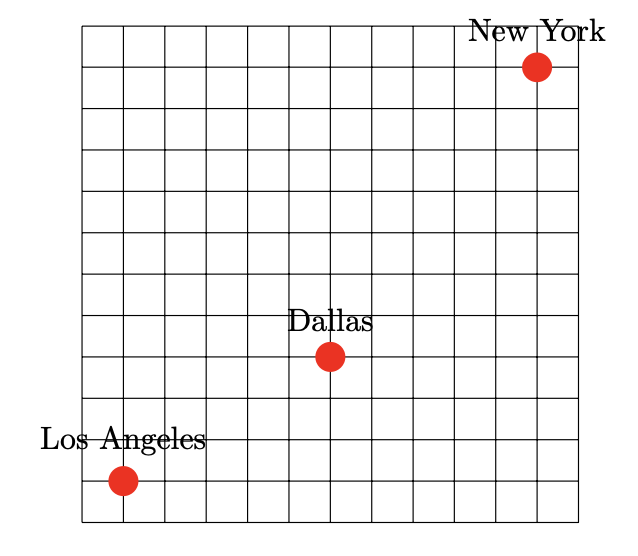
\includegraphics[width=0.4\textwidth]{tonystarkgrid.png}
    \label{fig:grid}
\end{figure}

If an Iron-Man tries to move off the grid or into an obstacle, it merely stays in place. Additionally, each step has a cost that depends on the robot's location. For example, moving left from $(0,1)$ might cost 1 fuel but moving left from $(10,15)$ might require jumping over someone's backyard pool and thus might cost 3 fuels. Once a robot reaches Stark Industries, it powers down and costs 0 fuels even as its counterpart continues to move. You are given the positions of Los Angeles $\left(x_{\ell}, y_{\ell}\right)$, Dallas $\left(x_d, y_d\right)$, and New York $\left(x_{n y}, y_{n y}\right)$, the positions of all obstacles $\left(x_{o_i}, y_{o_i}\right)$, and the cost of every possible move from every possible location.
    
\begin{enumerate}
    \item {\bf (10 points)} Give and explain an asymptotic upper bound on how many possible positions there are for the pair of Iron-Men, and explain why no better asymptotic upper bound is possible.
    \item {\bf (20 points)} Give an algorithm to find the cheapest sequence of $\{\mathrm{L}, \mathrm{R}, \mathrm{U}, \mathrm{D}\}$ moves (that is, the one that requires you to buy the smallest amount of robot fuel) that will bring both Iron-Men home to New York.
Hint: Try to represent the position of the two Iron-Men as a single vertex in some graph. For full credit, it suffices to find an $O\left(n^8\right)$ algorithm, but an $O\left(n^4 \log n\right)$ algorithm may be eligible for an exceptional score.
\end{enumerate}

(Note: You may find the question above more accessible after the Monday (Feb. 5) lecture.)

\item {\bf (0 points, optional)} This problem is based on the $2 \mathrm{SAT}$ problem. The input to $2 \mathrm{SAT}$ is a logical expression of a specific form: it is the conjunction (AND) of a set of clauses, where each clause is the disjunction (OR) of two literals. (A literal is either a Boolean variable or the negation of a Boolean variable.) For example, the following expression is an instance of 2SAT:
$$
\left(x_1 \vee \overline{x_2}\right) \wedge\left(\overline{x_1} \vee \overline{x_3}\right) \wedge\left(x_1 \vee x_2\right) \wedge\left(x_4 \vee \overline{x_3}\right) \wedge\left(x_4 \vee \overline{x_1}\right)
$$

A satisfying assignment to an instance of a 2SAT formula is an assignment of the variables to the values $\mathrm{T}$ (true) and $\mathrm{F}$ (false) so that all the clauses are satisfied- that is, there is at least one true literal in each clause. For example, the assignment $x_1=T, x_2=F, x_3=F, x_4=T$ satisfies the 2SAT formula above.

Derive an algorithm that either finds a satisfying assignment to a 2SAT formula, or returns that no satisfying assignment exists. Carefully give a complete description of the entire algorithm and the running time.

(Hint: Reduce to an appropriate problem. It may help to consider the following directed graph, given a formula $I$ in 2SAT: the nodes of the graph are all the variables appearing in $I$, and their negations. For each clause $(\alpha \vee \beta)$ in $I$, we add a directed edge from $\bar{\alpha}$ to $\beta$ and a second directed edge from $\bar{\beta}$ to $\alpha$. How can this be interpreted?)


\end{enumerate}



\end{document}
